% 
% Annual Cognitive Science Conference
% Sample LaTeX Paper -- Proceedings Format
% 

% Original : Ashwin Ram (ashwin@cc.gatech.edu)       04/01/1994
% Modified : Johanna Moore (jmoore@cs.pitt.edu)      03/17/1995
% Modified : David Noelle (noelle@ucsd.edu)          03/15/1996
% Modified : Pat Langley (langley@cs.stanford.edu)   01/26/1997
% Latex2e corrections by Ramin Charles Nakisa        01/28/1997 
% Modified : Tina Eliassi-Rad (eliassi@cs.wisc.edu)  01/31/1998
% Modified : Trisha Yannuzzi (trisha@ircs.upenn.edu) 12/28/1999 (in process)
% Modified : Mary Ellen Foster (M.E.Foster@ed.ac.uk) 12/11/2000
% Modified : Ken Forbus                              01/23/2004
% Modified : Eli M. Silk (esilk@pitt.edu)            05/24/2005
% Modified: Niels Taatgen (taatgen@cmu.edu) 10/24/2006

%% Change ``a4paper'' in the following line to ``letterpaper'' if you are
%% producing a letter-format document.

\documentclass[10pt,letterpaper]{article}

\usepackage{cogsci}
\usepackage{pslatex}
\usepackage{apacite}
\usepackage{graphicx}
\usepackage{float}
\usepackage{amsmath}

\title{The role of social cues to reference in cross-situational word learning}
 
\author{{\large \bf Kyle MacDonald (kyle.macdonald@stanford.edu)}} 


\begin{document}

\maketitle


\begin{abstract}
Social cues and statistical regularity are both rich sources of information for word learners. Past research shows that social interaction facilitates language acquisition \cite{baldwin1995understanding, brooks2008infant} and in the absence of social information adults and children can track co-occurrence information to learn words \cite{blythe2010learning,smith2008infants}.  In the current study, I explore the interaction between these two information sources with a behavioral experiment and a computational model. The model attempts to formalize the interaction between social information and the learner's strength of belief about referential intent to generate predictions about human behavior. The experiment adds a social cue (eye gaze) to a typical cross-situational word learning task, changing the ambiguity of the initial learning episode. I predicted that eye gaze would give learners more evidence about referential intent, allowing them to "explain away" spurious word-object mappings and reduce tracking of multiple referents for each word. Results suggest that learners were sensitive to the social cue, but did not change how they track multiple referents. Potential explanations for these results and future directions are discussed.  

\textbf{Keywords:} 
word learning; eye gaze; statistical learning; language acquisition
\end{abstract}


\section{Introduction}
To acquire a new word\footnote{Here I will focus on the task of mapping words to objects with the goal of learning concrete nouns and assume that the learner has already solved the problem of word segmentation.}, the learner must solve several problems. She must simultaneously infer what is being talked about and the meaning of individual words in the speaker's utterance. This joint inference problem can be divided into two parts. The first involves making an inference about speaker's referential intent and the second making an inference about the links between words and objects. Together, these social-cognitive and mapping challenges make word learning a surprisingly difficult puzzle for the child to solve, and a great deal of research has tried to explain how children can learn words so rapidly.

To account for children's word learning skills, different theories of language acquisition emphasize different tools and information sources available to the learner. These proposals can be divided into two broad categories: \emph{Social-Pragmatic} and \emph{Associative} accounts. Social-Pragmatic theories suggest that word learning occurs as a result of children's social-cognitive skills and the highly structured learning moments created by adults (i.e. joint attentional frames).  Both experimental and observational data show that children possess sophisticated intention-reading skills, which they use in the service of word learning \cite{baldwin1993infants} and that episodes of joint attention facilitate word learning and vocabulary growth \cite{brooks2008infant}.  

In contrast, Associative accounts highlight the powerful statistical learning mechanisms that allow learners to track the regularities of language. In this account, word learning is best explained by domain-general pattern-finding abilities, attention, and memory. Several studies show In the absence of social cues to word meaning, adults and children are able to rapidly learn words by tracking the co-occurrence statistics of labels and objects across exposures \cite{smith2008infants,vouloumanos2008fine}. However, some researchers question the psychological plausibility of gradualist accounts, arguing that children's rapid word learning is better described by a single hypothesis tracking mechanism \cite{trueswell2013propose,medina2011words}. 

Recent experimental and modeling work suggests that learners track both a single, strong hypothesis and multiple referents, providing evidence for an integrated account of cross-situational learning (Yurovsky & Frank, in prep). In Yurovsky and Frank's task, participants saw a set of novel objects and heard a novel word (e.g. Grink), and were asked to make a guess about the "correct"\footnote{There was actually no "correct" answer on exposure trials; rather these trials gave participants evidence about potential word-object mappings and allowed them to form an initial hypothesis.} word-object mapping. In subsequent test trials, participants heard the novel word again, this time paired with another set of novel objects. Critically, one of the objects in the new set was either the participant's initial hypothesis (Same trials) or one of the objects that was \emph{not} the initial hypothesis (Switch trials). On Switch trials, adults reliably selected the object that was not their initial hypothesis, even when there were eight objects in the initial exposure set, providing strong evidence that learners track multiple referents when learning from ambiguous contexts.

However, this task did not include any of the rich social cues that typically accompany real world word learning. So it is still an open question as to how social information interacts with learners' demonstrated ability to track multiple referents. Perhaps the presence of additional evidence about a speaker's referential intent strengthens the learner's initial hypothesis, reducing the need to track alternative hypotheses. Or it could be that social information strengthens the initial hypothesis without reducing multiple referent tracking. The current study follows a recent line of empirical work and modeling that attempts to integrate statistical and social learning\cite{johnson2012exploiting,frank2009using,yu2007unified}, and asks if the presence of social information changes how learners track multiple referents when learning new words.

\begin{figure*}
	\centering
	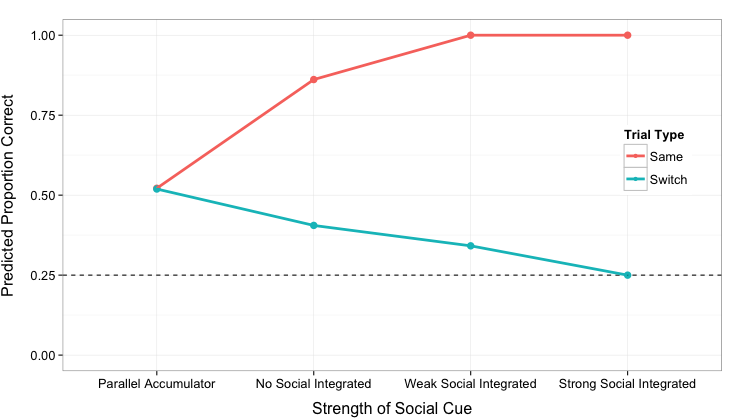
\includegraphics[scale=0.5]{model_predictions.png}
	\caption{Model predictions of performance on Same and Switch trials. The ability of social information to influence the learner's beliefs about referential intent is captured by the $\sigma$ parameter, which in turn directly influences the strength of initial encoding. The Parallel Accumulator, which allocates belief equally across all objects, and the No Social parameter values were taken from Yurovsky and Frank (in prep). The model predicts that as the speaker's intention becomes more obvious, performance on Same trials reaches ceiling and performance on Switch trials declines. This is because the learner is allocating all of the probability mass to one referent: the target of the speaker's referential intent.}
\end{figure*}

\section{Model}

First, I begin by describing the computational model developed by \citeA{frank2009using} and extended by Yurovsky and Frank (in prep). Then, I will discuss how I modified the model's parameters in order to generate predictions about the effect of social cues to reference on cross-situational learning. 

In \citeauthor{frank2009using}'s model, the word-learning problem is defined by a set of variables and probabilistic dependencies that link these variables. The learner observes a set of situations \emph{S}, which consist of two observed variables - objects (\emph{O}) and words (\emph{W}) - and one hidden variable: the speaker's intention (\emph{I}), with the goal of inferring the most probable lexicon of word-object mappings (\emph{L}) given the set of observed situations. Formally, the task of learning the correct lexicon can be defined as a problem of Bayesian inference: 
%
\begin{equation}
\label{1}
P(L|S) \propto P(S|L)P(L)
\end{equation}
%
The likelihood term ($P(S|L)$) captures the learner's assumptions about the task. Each situation (\emph{S}) includes a word, a set of objects, and the speaker's referential intention (\emph{I}). Thus, $P(S|L)$ can be expanded and the probability of the lexicon can be given as: 
%
\begin{equation}
\label{2}
P(L|S) \propto \prod\limits_{s \in S}  P(W_s, I_s, O_s|L)P(L)
\end{equation}
%
Because referential intention mediates the relationship between words and objects, the likelihood term can be rewritten as:
%
\begin{equation}
\label{3}
P(L|S) \propto \prod\limits_{s \in S}  P(W_s|I_s, L)P(I_s|O_s)P(L)
\end{equation}
%
The prior probability of a lexicon is defined as: $P(L_o) \propto \frac{1}{|L_o|}$, which is a parsimony prior that favors lexicons with fewer words referring to the same object. 

Thus far, I have described the computational problem for the Bayesian word learner outlined by \citeNP{frank2009using}. Yurovsky and Frank then extended this computational level description to include cognitive constraints (memory and attention), allowing them to provide an algorithmic-level account of their data. Memory was modeled as a power function that took into account the interval between successive exposures to a word. The $\gamma$ parameter scaled to the strength of the initial encoding and the $\lambda$ parameter defined the rate of decay.
%
\begin{equation}
\label{4}
M(L_o) =  \gamma L_ot^{-\lambda}
\end{equation}
%

Attention was defined in terms of the learner's belief about $P(I|O)$: the probability of the speaker's intention to refer to each object in the set. The $\sigma$ parameter captures the amount of probability mass that the learner  places on each referent during the initial exposure. The strength of the learner's belief about $P(I|O)$ in turn directly influences the strength of initial encoding. At $\sigma = 1$, the learner is placing all of the probability mass on one word-object mapping (i.e. a single hypothesis tracking strategy). At $\sigma = \frac{1}{|O|}$, the learner is distributing the probability mass across all possible word-object mappings equally (i.e. a parallel statistical accumulator strategy). 

Figure 1 shows model predictions for four different levels of belief about referential intent (i.e. four different values for $\sigma$). The first two models are from Yurovsky and Frank (in prep). The Parallel Accumulator model, $\sigma = (\frac{1}{|\sigma|})$, predicts indistinguishable performance on Same and Switch trials because the learner is allocating belief evenly across referents. The No Social Integrated model predicts strong performance on Same trials and above chance performance on Switch trials because it allocates a chunk of probability to a single hypothesis and distributes the rest to the other referents. This model was the best fit for human behavior on their cross-situational learning task, explaining 98\% of the variance in the data. 

However, these two models did not include the rich social cues to reference that are available to the word learner. Perhaps more evidence about referential intent will cause the learner to place more belief on the object that is the target of the referential act. To formalize this intuition, I modified the $\sigma$ parameter in Frank and Yurovsky's model to generate predictions about human performance on a social, cross-situational learning task (see Figure 1). The Weak Social model treats social information as additional evidence about reference, and increases the allocation of belief to a single hypothesis, $\sigma = 0.75$. It predicts an improvement on Same trials and a decrease in performance on Switch trials. However, the learner still tracks multiple referents and does not place \emph{all} belief on a single hypothesis. In contrast, the Strong Social model ($\sigma = 1$) predicts that learners will not track multiple referents because all of their probability mass is allocated entirely to the target of the speaker's referential intent, similar to the single-hypothesis tracking strategy suggested by Trueswell and colleagues. 

Next, I describe an experiment that explores these predictions in a cross-situational learning task that includes social cues to reference. Will social information shift learners to a single-hypothesis tracking strategy? Or will learners still track multiple hypotheses despite the additional evidence about referential intent?

\section{Experiment}

\subsection{Participants}

This experiment was posted to Amazon Mechanical Turk as a set of
Human Intelligence Tasks (HITs) to be completed only by participants with US IP
addresses that paid 30 cents each (for a detailed comparison of laboratory and Mechanical
Turk studies see \citeNP{crump2013evaluating}). 30 HITs were posted for each
condition (Social, Non-social) for total of 60 paid HITs. If a participant
completed the experiment more than once, he or she was paid each time but only data
from the first HITs completion was included in the final data set. In
addition, data was excluded from the final sample if participants did not give correct
answers for familiar trials (excluded 1 HIT).

\subsection{Stimuli}

Stimuli for the experiment consisted of black and white pictures of familiar
and novel objects, a schematic drawing of a human interlocutor, and audio recordings of familiar and novel words. Pictures of 32 familiar objects spanning a range of categories (e.g. squirrel, truck, tomato, sweater) were drawn from the set constructed by \citeA{snodgrass1980standardized}. Pictures of distinct but
difficult to name objects were drawn from the set of 140 first used in \citeA{kanwisher1997locus}. For ease of viewing on participants' monitors, pixel values for all pictures were inverted so that they appeared as white outlines on black backgrounds (see Figure 1). Familiar words consisted of the labels for the familiar objects as produced by AT&T Natural VoicesTM (voice: Crystal). Novel words were 1-3 syllable pseudowords obeying the rules of English phonotactics produced using the same speech synthesizer.
%
\begin{figure}
	\centering
	\fbox{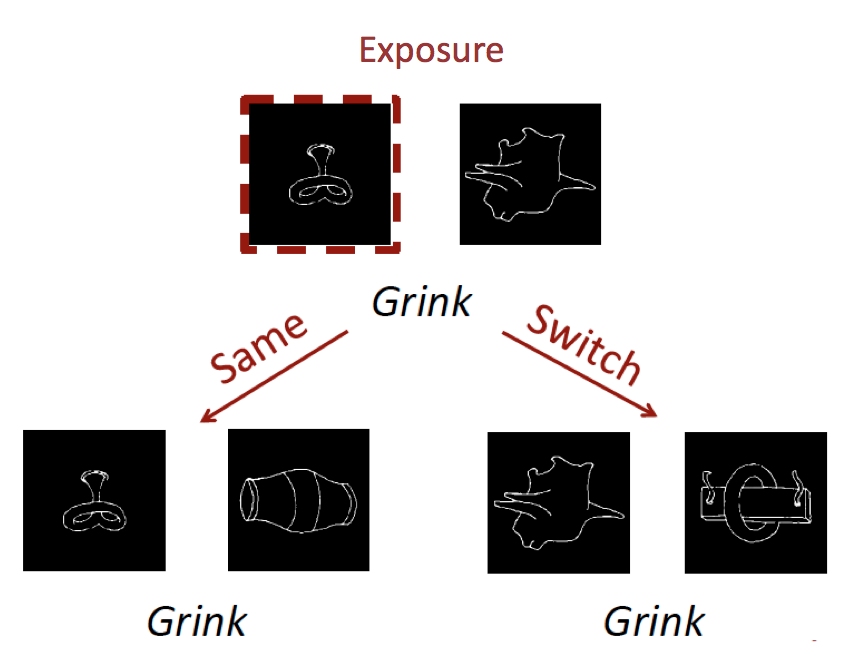
\includegraphics[scale=0.22]{stimuli2.png}}
	\caption{A schematic of the trials that participants saw in the experiment. On Exposure trials, participants saw four novel objects and heard a novel word. Participants were asked to guess it's correct referent. After the Exposure trial, participants either saw a Same or a Switch trial. On Same trials, the set of four referents contained the participant's previous hypothesis. On Switch trials, the set of referents contained one of the objects that the participants had \emph{not} hypothesized.}
\end{figure}

A schematic drawing of a human interlocutor was chosen for ease of manipulating the direction of eye gaze, the social cue of interest in this study. Five images were created using Adobe Photoshop with the following directions of eye gaze: far left, close left, close right, far right, and eyes center. Because this task was performed over the internet and participants' screen sizes might be small, it was important to make the eye gaze cue clear.
%
\begin{figure}
	\centering
	\fbox{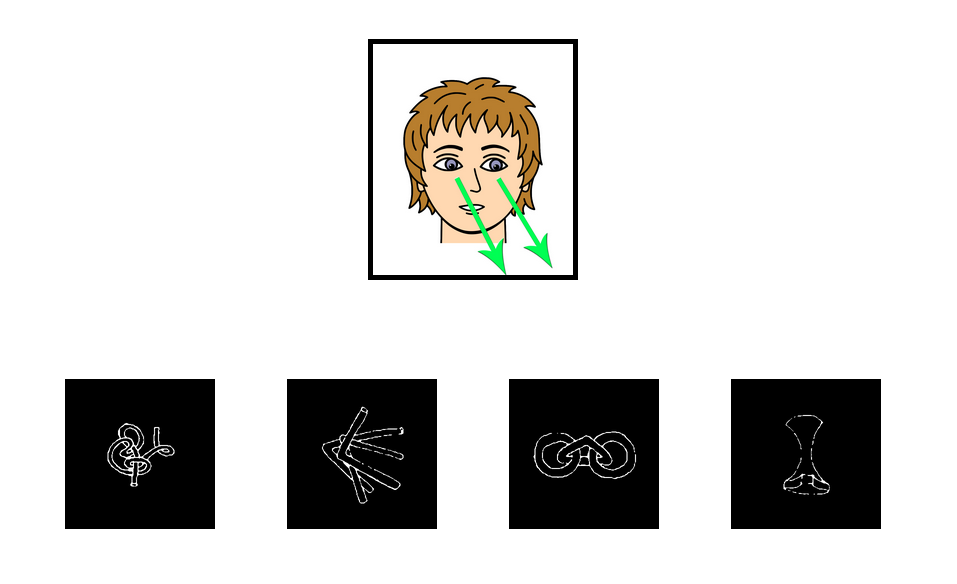
\includegraphics[scale=0.2]{stimuli1.png}}
	\caption{Exposure trials in the Social condition. In the Nonsocial condition, the interlocutor looked straight ahead during exposure. During test trials, the interlocutor looked straight ahead.}
\end{figure}
%
\subsection{Design and Procedure}
Participants were exposed to a series of trials in which they heard an interlocutor say a novel word, saw
four novel objects, and were asked to indicate their guess as to which object was the
referent of the word. After a written explanation of this procedure, participants were given
four practice trials to introduce them to the task. On each of these trials, they heard the interlocutor say a
Familiar word while looking at a line drawing of that object among a set of other familiar objects.
On the first two trials, participants were asked to find the squirrel, and the correct answer
was in the same position on each trial. On the next two trials, participants were asked to
find the tomato, and the correct answer switched positions from the first to the second
trial (in order to ensure that participants understood that the on-screen position was not
an informative cue to the correct target). These trials also served to screen for participants
who did not have their audio enabled or who were not attending to the task.

After these Familiarization trials, participants were informed that they would now hear
novel words, and see novel objects, and that they should continue selecting the correct
referent for each word. Participants each heard eight novel words twice. Participants saw four referents
on each trial, and the two trials for each word occurred back-to-back. Four of these
follow-up trials were Same trials in which the referent that participants selected on the exposure trial appeared again amongst the set of objects. The other four were
Switch trials in which one of the referents in the set was selected randomly from the objects
a participant did not select on the previous Exposure trial. All other referents were
completely novel on each trial. Critically, on Exposure trials the interlocutor's eye gaze was directed and thus informative, but on Same/Switch trials her eye gaze was undirected and thus uninformative. 

Participants were randomly assigned to one of two conditions: Social or Nonsocial. In the Social condition, eye gaze was informative on exposure trials. In the Nonsocial condition, eye gaze was uninformative throughout the task, i.e. the speaker always looked straight ahead. 

Because participants performed this task over the internet, it was important to
indicate to them that their click had been registered. Thus, a red dashed box appeared
around the object they selected for 1 second after their click was received. This box
appeared around the selected object whether or not it was the "correct" referent.

\section{Results and Discussion}

First, I compared the distribution of correct\footnote{A correct response for Same/Switch trials was selecting the referent that was present during Exposure trials.} responses to the distribution expected if participants were randomly selecting (defined by a Binomial distribution with four trials and a probability of success of $\frac{1}{\#Referents}$). Figure 4 shows participants' accuracy in identifying the correct referent for each word in both conditions for each trial type (Same and Switch). For all trial types and conditions, participants' responses differed from those expected by chance (smallest $\chi^{2}(4) = 12.07, p < .01$), replicating Yurovsky and Frank's finding that adults encode more than a single hypothesis in ambiguous cross-situational learning. 

\begin{figure}[H]
	\centering
	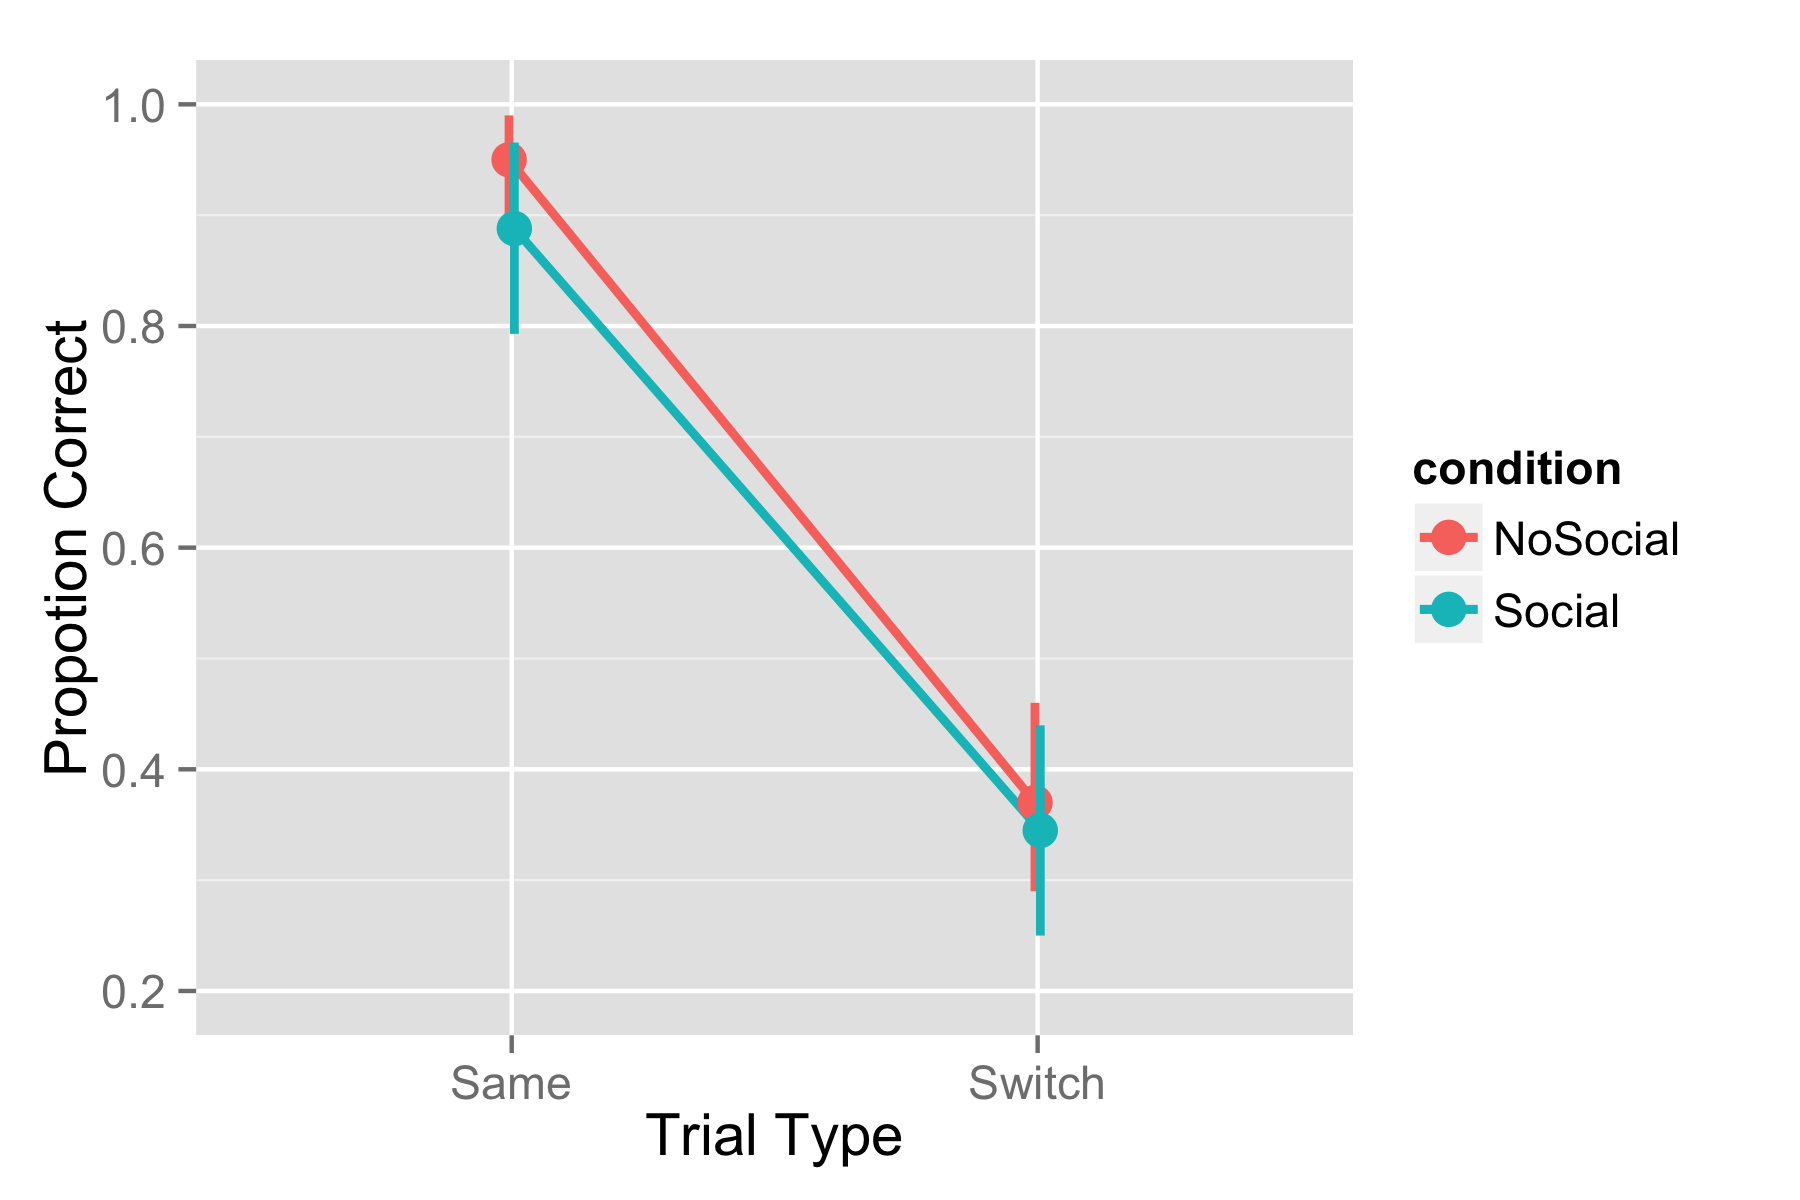
\includegraphics[scale=0.15]{accuracydark.png}
	\caption{Proportion of repeated referents selected by participants for each trial type (Same/Switch) and condition (Social/Nonsocial). Error bars indicate 95\% confidence intervals. Learning in all conditions differed from chance. There was no difference between the Social and Nonsocial conditions.}
\end{figure}

Next, I analyzed participants' accuracy on Same/Switch trials across conditions. A two-way analysis of variance with two levels of trial type (Same, Switch) and condition (Social, Nonsocial) yielded a significant main effect of trial type, $F(1, 104) = 167.36, p < .001$, such that participants were more accurate on Same trials ($M = \%91.6$) compared to Switch trials ($M = \%35.6$). There was no main effect of condition, $F(1, 104) = 0.05, p > .05$, and the interaction term was not significant, $F(1, 104) = 0.009, p > .05$.  Thus, I did not find evidence that social cues change how participants tracked and recalled multiple referents on subsequent test trials.

To check if participants were actually sensitive to the speaker's eye gaze, I compared the distribution of correct responses\footnote{A correct response on Exposure trials is selecting the referent that was the target of the speaker's eye gaze.} on Exposure trials to the distribution expected if participants were selecting randomly (defined by a Binomial distribution with one trial and a probability of success of $(\frac{1}{\#Referents}$). Participants' responses differed from those expected by chance, exact binomial $p(two-tailed) < .001$, suggesting that they were sensitive to and able to use the social cue.

Finally, I explored participants' reaction times, comparing across conditions to see if the presence of social information altered the rate of responses. Figure 4 shows participants' reaction time by trial and condition. A two-way analysis of variance with two levels of trial type (Same, Switch) and condition (Social, Nonsocial) yielded a significant main effects of trial type and condition, both p < .01, such that participants were faster in the Nonsocial condition and on Same trials. The interaction term was not significant, $F(1, 104) = 0.20, p > .05$.  Thus, I did not find evidence that the presence of social information during exposure trials changes the rate of participants' responses. 

\begin{figure}[H]
	\centering
	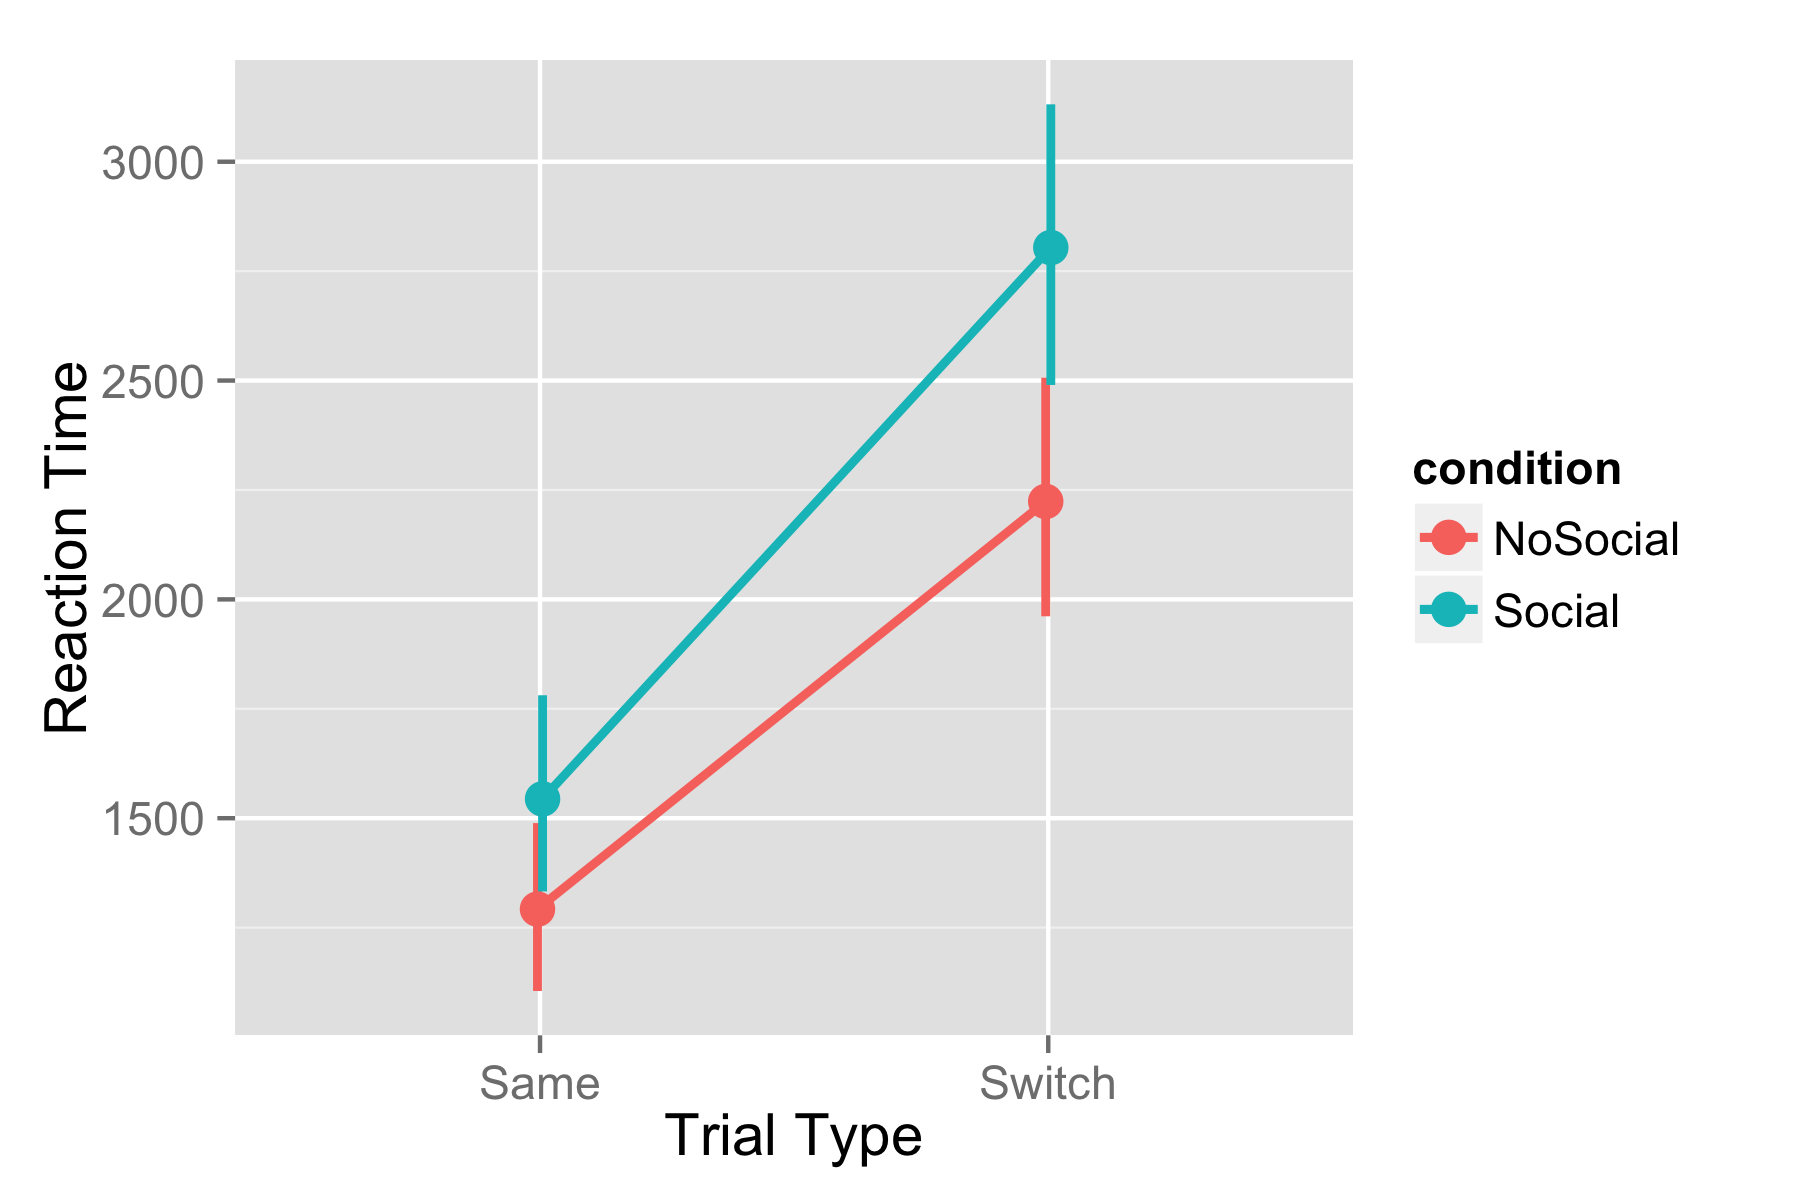
\includegraphics[scale=0.15]{rt.png}
	\caption{Reaction time for each trial type (Same/Switch) and condition (Social/Nonsocial). Error bars indicate 95\% confidence intervals. Participants were slower on Switch trials and in the Social condition. The interaction between trial type and condition was not significant.}
\end{figure} 

Together, these results suggest that participants were sensitive to the social cue manipulation, selecting the target of the interlocutor's gaze on Exposure trials. However, this sensitivity did not did not change how participants performed on accuracy or reaction time in either Same/Switch trials. Potential explanations for these results and future directions are discussed below. 

\section{Conclusions and future work}

In this paper, I explored the interaction of social and statistical information during cross-situational word learning. First, I described a computational model that builds off recent empirical and modeling work (\citeNP{frank2009using}, Yurovsky & Frank, in prep) and attempts to integrate the computational problem of cross-situational word learning with psychological constraints and social information. I generated predictions from this model by modifying the proportion of probability mass allocated to a single or multiple referents based on assumptions about how social cues might influence learners' beliefs. Finally, I presented empirical work that investigated whether the presence of social information would change how adults track multiple word meanings. 

I predicted that eye gaze would provide additional evidence about a speaker's referential intent, strengthening the learner's initial hypothesis, potentially at a cost to tracking alternative hypotheses (similar to the predictions made by the Weak Social cue model). The results did not provide evidence in support of this prediction: adults tracked multiple hypotheses regardless of the presence of a social cue. 

So why might learners continue to track multiple hypotheses, even when they have stronger evidence about the correct word-object mapping during exposure? The analysis of performance on Exposure trials rules out the alternative explanation that participants did not pay attention to the social cue. However, it is possible that the combination of a static/schematic interlocutor and the lack of a natural sentence frame (e.g. "There's a X") caused the task to be pragmatically strange, which might have led participants to discount the interlocutor as a source of evidence about word-object mappings. 

It could be that limiting the social information to eye gaze resulted in a weak social cue that wasn't strong enough to change how learners tracked referents. Recent research suggests that eye gaze might be a noisy and unreliable cue in natural learning environments \cite{frank2013social}. Future versions of the task could include stronger cues such as pointing or holding the object to see if stronger evidence would alter referent tracking. Future versions could also include more complex Exposure trials and more trials between exposure and test (similar to Yurovsky & Frank, in prep) to see how social information interacts with attention and memory demands. 

Another interesting possibility is that participants did not treat the interlocutor as a reliable information source. Within the first two trials of the experiment, participants are given strong negative evidence about the reliability of the interlocutor's gaze. That is, on Switch trials, the target of gaze (and the participant's initial hypothesis) is all of sudden no longer present on the screen. It is plausible that one piece of strong negative evidence is enough to cause the learner to pay more attention to the other referents in subsequent trials. Future versions could establish the reliability of the speaker's gaze by first presenting a block of Same trials and then measuring how participants' referent tracking behavior changes as Switch trials are introduced. More work is needed to tease apart these potential explanations for participants' behaviors on this task.

Language learning involves solving several complex inference problems. Thus, it is likely that language learners use several tools to take advantage of the sources of information available to them, both social and statistical. This study follows recent work that attempts to integrate social and statical learning approaches with the hope that future studies will increase our understanding of the unique contribution of each and how they interact to support learning. 

\bibliographystyle{apacite}

\setlength{\bibleftmargin}{.125in}
\setlength{\bibindent}{-\bibleftmargin}

\bibliography{fyp_p}


\end{document}
